
% Template for Elsevier CRC journal article
% version 1.2 dated 09 May 2011

% This file (c) 2009-2011 Elsevier Ltd.  Modifications may be freely made,
% provided the edited file is saved under a different name

% This file contains modifications for Procedia Computer Science

% Changes since version 1.1
% - added "procedia" option compliant with ecrc.sty version 1.2a
%   (makes the layout approximately the same as the Word CRC template)
% - added example for generating copyright line in abstract

%-----------------------------------------------------------------------------------

%% This template uses the elsarticle.cls document class and the extension package ecrc.sty
%% For full documentation on usage of elsarticle.cls, consult the documentation "elsdoc.pdf"
%% Further resources available at http://www.elsevier.com/latex

%-----------------------------------------------------------------------------------

%%%%%%%%%%%%%%%%%%%%%%%%%%%%%%%%%%%%%%%%%%%%%%%%%%%%%%%%%%%%%%
%%%%%%%%%%%%%%%%%%%%%%%%%%%%%%%%%%%%%%%%%%%%%%%%%%%%%%%%%%%%%%
%%                                                          %%
%% Important note on usage                                  %%
%% -----------------------                                  %%
%% This file should normally be compiled with PDFLaTeX      %%
%% Using standard LaTeX should work but may produce clashes %%
%%                                                          %%
%%%%%%%%%%%%%%%%%%%%%%%%%%%%%%%%%%%%%%%%%%%%%%%%%%%%%%%%%%%%%%
%%%%%%%%%%%%%%%%%%%%%%%%%%%%%%%%%%%%%%%%%%%%%%%%%%%%%%%%%%%%%%

%% The '3p' and 'times' class options of elsarticle are used for Elsevier CRC
%% The 'procedia' option causes ecrc to approximate to the Word template
\documentclass[3p,times,procedia]{elsarticle}
\flushbottom

%% The `ecrc' package must be called to make the CRC functionality available
\usepackage{ecrc}
\usepackage{multirow}
\usepackage{comment}
%\usepackage{amsmath}


%% The ecrc package defines commands needed for running heads and logos.
%% For running heads, you can set the journal name, the volume, the starting page and the authors

%% set the volume if you know. Otherwise `00'
\volume{00}

%% set the starting page if not 1
\firstpage{1}

%% Give the name of the journal
\journalname{Procedia Computer Science}

%% Give the author list to appear in the running head
%% Example \runauth{C.V. Radhakrishnan et al.}
\runauth{A. Karapetyan, W. Yaqub et al.}

%% The choice of journal logo is determined by the \jid and \jnltitlelogo commands.
%% A user-supplied logo with the name <\jid>logo.pdf will be inserted if present.
%% e.g. if \jid{yspmi} the system will look for a file yspmilogo.pdf
%% Otherwise the content of \jnltitlelogo will be set between horizontal lines as a default logo

%% Give the abbreviation of the Journal.
\jid{procs}

%% Give a short journal name for the dummy logo (if needed)
%\jnltitlelogo{Procedia Computer Science}

%% Hereafter the template follows `elsarticle'.
%% For more details see the existing template files elsarticle-template-harv.tex and elsarticle-template-num.tex.

%% Elsevier CRC generally uses a numbered reference style
%% For this, the conventions of elsarticle-template-num.tex should be followed (included below)
%% If using BibTeX, use the style file elsarticle-num.bst

%% End of ecrc-specific commands
%%%%%%%%%%%%%%%%%%%%%%%%%%%%%%%%%%%%%%%%%%%%%%%%%%%%%%%%%%%%%%%%%%%%%%%%%%

%% The amssymb package provides various useful mathematical symbols

\usepackage{amssymb}
%% The amsthm package provides extended theorem environments
%% \usepackage{amsthm}

%% The lineno packages adds line numbers. Start line numbering with
%% \begin{linenumbers}, end it with \end{linenumbers}. Or switch it on
%% for the whole article with \linenumbers after \end{frontmatter}.
%% \usepackage{lineno}

%% natbib.sty is loaded by default. However, natbib options can be
%% provided with \biboptions{...} command. Following options are
%% valid:

%%   round  -  round parentheses are used (default)
%%   square -  square brackets are used   [option]
%%   curly  -  curly braces are used      {option}
%%   angle  -  angle brackets are used    <option>
%%   semicolon  -  multiple citations separated by semi-colon
%%   colon  - same as semicolon, an earlier confusion
%%   comma  -  separated by comma
%%   numbers-  selects numerical citations
%%   super  -  numerical citations as superscripts
%%   sort   -  sorts multiple citations according to order in ref. list
%%   sort&compress   -  like sort, but also compresses numerical citations
%%   compress - compresses without sorting
%%
%\biboptions{sort&compress}

% \biboptions{}

% if you have landscape tables
\usepackage[figuresright]{rotating}
%\usepackage{harvard}
% put your own definitions here:x
%   \newcommand{\cZ}{\cal{Z}}
%   \newtheorem{def}{Definition}[section]
%   ...

% add words to TeX's hyphenation exception list
%\hyphenation{author another created financial paper re-commend-ed Post-Script}

% declarations for front matter

\begin{document}

\begin{frontmatter}

%% Title, authors and addresses

%% use the tnoteref command within \title for footnotes;
%% use the tnotetext command for the associated footnote;
%% use the fnref command within \author or \address for footnotes;
%% use the fntext command for the associated footnote;
%% use the corref command within \author for corresponding author footnotes;
%% use the cortext command for the associated footnote;
%% use the ead command for the email address,
%% and the form \ead[url] for the home page:
%%
%% \title{Title\tnoteref{label1}}
%% \tnotetext[label1]{}
%% \author{Name\corref{cor1}\fnref{label2}}
%% \ead{email address}
%% \ead[url]{home page}
%% \fntext[label2]{}
%% \cortext[cor1]{}
%% \address{Address\fnref{label3}}
%% \fntext[label3]{}

\dochead{6th International Conference on Ambient Systems, Networks and Technologies, ANT 2015 and the 5th International Conference on Sustainable Energy Information Technology, SEIT 2015}
%% Use \dochead if there is an article header, e.g. \dochead{Short communication}
%% \dochead can also be used to include a conference title, if directed by the editors
%% e.g. \dochead{17th International Conference on Dynamical Processes in Excited States of Solids}

\title{A Two-Stage Comparative Life Cycle Assessment of Paper-Based and Software-Based Business Cards}

%% use optional labels to link authors explicitly to addresses:
%% \author[label1,label2]{<author name>}
%% \address[label1]{<address>}
%% \address[label2]{<address>}


\author{Areg Karapetyan \corref{cor1}}
\ead{akarapetyan@masdar.ac.ae}
\author{Waheeb Yaqub \corref{cor1}}
\ead{wyaqub@masdar.ac.ae}
\author{Aram Kirakosyan}
\ead{akirakosyan@masdar.ac.ae}
\author{Sgouris Sgouridis}
\ead{ssgouridis@masdar.ac.ae}

\address{Department of Electrical Engineering and Computer Science, Masdar Institute of Science and Technology, Abu Dhabi, UAE}



\begin{abstract}
%% Text of abstract
Information and digital communication technologies are playing an important role in shaping the future of communities and societies. Identifying the environmental impacts of digital products and services is helpful for taking sustainable decisions. This article introduces the findings of a comparative life cycle assessment of two business card options: a smartphone software and the common paper-based alternative. Life cycle burdens of the production, distribution and use of business cards were compared and contrasted for both systems. Furthermore, as far as we have been able to determine, there has been no study evaluating the environmental impacts of software-based (digital) and paper-based business cards. Given the prevalence and multifunctionality of digital devices and services, this paper analyzes the environmental impacts and impact categories of the two systems as well as evaluates their total energy consumption, Green House Gas (GHG) emissions and toxic releases by conducting a two-stage life cycle assessment with alternating functional units. The results indicate that, for a small scale functional unit, the paper-based business card system causes slightly less environmental impact and has lower energy demand than the digital business card system. Whereas when considering a large scale (real world scenario) functional unit, the digital business card system is more environmentally friendly and economical in terms of energy consumption. By comparing these two systems, this paper could serve businesses and consumers as a basis for considering environmental consequences and energy depletion regarding the two business card options.
\end{abstract}


\begin{keyword}
Life Cycle Assessment; Information and Communication Technologies; Internet; Environmental Impact; Input-Output Life Cycle Assessment; Printed Business Cards; Digital Business Cards; 

%% keywords here, in the form: keyword \sep keyword

%% PACS codes here, in the form: \PACS code \sep code

%% MSC codes here, in the form: \MSC code \sep code
%% or \MSC[2008] code \sep code (2000 is the default)

\end{keyword}
\cortext[cor1]{Corresponding author. Tel.: +971-56-953-6068, +971-55-345-7753 }
\end{frontmatter}

%\correspondingauthor[*]{Corresponding author. Tel.: +0-000-000-0000 ; fax: +0-000-000-0000.}
%\email{akarapetyan@masdar.ac.ae, wyaqub@masdar.ac.ae }

%%
%% Start line numbering here if you want
%%
% \linenumbers

%% main text

%\enlargethispage{-7mm}
\section{Introduction}

Human originated impacts on climate variation, increased consumption of natural resources, specifically fossil fuels, as well as the harmful consequences of industrial pollution have drawn global consciousness to the concepts of sustainability -welfare of future generations and life cycle thinking, which significantly constrained not only industrial and commercial sectors of the global economy, but also routine activities in terms of energy and resource consumption and environmental footprint. At the same time, thanks to the rapid growth of the World Wide Web (Internet) and advances in digital technologies over the past decade, the information and communication technologies (ICT) sector is revolutionizing and modifying the pathways of both human activity and the global economy. One of the most distinguishable transitions is that from paper to digital based systems. Nowadays, paper based products and services such as invoices, billing systems, teaching aids, books, magazines and newspapers, diaries, business cards and office documentation all have their digital alternatives.\\

Comparative analysis of the environmental impacts of traditional paper based products and their corresponding ICT enabled digital counterparts has been a subject of a  considerable body of research. These studies include but are not limited to comparison of digital and paper media, digital and print libraries, electronic and paper billing methods, printed and electronic teaching aids, printed newspaper, Internet newspaper and TV broadcast, online and paper based telephone directories, e-mail and traditional postal mail service, as well as printed scholarly books and e-book reading devices \cite{Bull201410, 6360455, enroth2009, zurkirch2000, kozak2003,hischier2003m}. However, despite the wide usage and high popularity of business cards (a card bearing business information about a company or individual) intended for promoting a person or business nowadays, to the best of our knowledge, information and data associated with the environmental effects and energy consumption during creation and usage of paper based business cards (PBC) and digital business cards (DBC) has not been well studied and quantified. The term PBC in this paper is referred as a white or full color paper stock having printed text and/or image(s) representing information about a business or a person. Likewise, the term DBC refers to a digital data containing information regarding a business or person stored in a local storage of a smartphone and accessible as a visualization. In fact, according to a CNN report and a number of Internet resources, in 2012 the annual number of printed business cards was estimated to be 10 billion.\\

Various research studies indicate that impressive rates of growth of technological advances and innovations have empowered the ICT sector with enough potential for reducing global energy and resource consumption and GHG emissions  \cite{10046363,924525, 6360455}. According to some technical reports \cite{s3758490, 7282419}, further modified ICT applications could save up to 7.8 GtCO2e, or 15\% of global CO2 equivalent emissions by 2020. From an economic perspective, this is synonymous to approximately \$743 billion of cost savings in terms of energy conservation.\\

Notwithstanding, the ICT sector itself challenges the environment and global energy reserves, which in combination with the tremendous rate of growth of this industry, contributes to the growing concerns about environmental impacts of ICT. A number of studies aimed at modeling, evaluating and identifying the direct and indirect influence of ICT applications on the global economy and environment, show that, because of its intermittent, extremely vague and interrelated nature, it is possible that ICT could have undesirable effects on the environment  \cite{Hilty20061618, 6083606, Bull201410}. According to the report conducted in 2009 \cite{7282419}, a typical Google search performed from a desktop computer can produce about 7g of CO2 per search. Considering that there are 3.5 billion Google searches per day on average, the resulting aggregate CO2 emissions only from this activity amounts to 24.5 KtCO2 per day, which is equivalent to the CO2 emissions from 2 million second generation 2004 Toyota Prius vehicles having a run of 100 km (based on the assumption that a second generation 2004 Toyota Prius vehicle emits 118.84 $\frac{g}{km}$ \cite{6728838}). In 2002, the ICT sector's total contribution to global GHG emissions was estimated to be 530 MtCO2e, whereas in 2007, the emissions increased to 620 MtCO2e (1.3\% increase) of the cumulative global GHG emissions. It has been forecasted that by 2020, ICT could cause GHG emissions of the order of 1.43 GtCO2e  \cite{malmodin2013future, s3758490}.\\

The ever increasing rate of growth of ICT applications and the aforementioned calculations demonstrate that quantifying and evaluating the direct environmental footprint of ICT applications is of crucial importance in terms of environmental preservation. Life Cycle Assessment (LCA), a widely used concept and technique for evaluating the environmental effects of a product or activity holistically has been considered in this study. According to ISO 14040 standard ``an LCA study analyzes the environmental aspects and potential environmental impacts throughout a product's life cycle, that is, from raw material acquisition through production, use, end-of-life treatment, recycling and final disposal (i.e. cradle-to-grave) of the product'' \cite{ISO140402006}.\\

This study, by performing a two-stage cradle-to-grave LCA analysis, compares paper-based and digital business card systems in terms of their environmental impacts and energy utilization. Contributions and findings of this paper present a comprehensive investigation of environmental impacts and impact categories of two systems as well as assesses their energy utilization, GHG emissions and toxic releases. The results provide businesses and consumers with viable and sufficient information to consider environmentally aware decisions regarding paper-based and digital business card option.


\section{Background and Related Work} 

Among various assessment techniques that fulfill the objective of measuring a product's or a service's environmental impact, ISO LCA\cite{ISO140402006}, Environmental Product Declarations (EPD)\cite{iso2006environmental} and PAS 2050 \cite{pas20082050} tend to be the most acknowledged, based on the literature review conducted in the scope of this study. Even though EPD provides with inclusive environmental impact evaluation tool that also identifies enhancement prospects, it overlooks certain problems such as carbon storage and the end-of-life phase. Unlike ISO LCA, PAS 2050 standards take into account only a solitary environmental aspect, namely, carbon footprint i.e. total GHG emissions, which makes this technique inflexible and inefficient in terms of identification and assessment of potential trade-offs. It's reasonable to argue that the comparison of two different products' impacts on the environment in terms of only GHG emissions will be less comprehensive and insightful compared to the holistic environmental impact comparison considering the factors that include but are not limited to toxic releases, ozone depletion and resource consumption. ISO LCA is widely accepted and  possesses capabilities to assess various environmental impacts of products and services \cite{cooper2006life}. Furthermore,  ISO 14000 family, so far, is the unique international standard document on LCA and is referenced by other standardization processes \cite{finkbeiner201340s}.\\

Inclusiveness of the LCA method through cradle-to-grave approach and the subsequent circumvention of problem shifting between influences and areas are indicated in \cite{hermann2007assessing} as some of the powerful aspects of LCA methodology. As stated by \cite{guldbrandsson2012opportunities} a number of companies including Ericsson telecom company acknowledges LCA methodology as a worthwhile and suitable framework for evaluating and labeling their products' eco-friendliness. Furthermore, \cite{finnveden2000limitations} compares LCA and Environmental Systems Analysis(ESA) tools in general, and concludes that, LCA is the best option if the objective is to examine the environmental burdens caused by a product or a service.\\

Although LCA has promising capabilities, it has weaknesses and limitations with its methodological framework. Several authors that include but not limited to \cite{joshi1999product, reap2008survey, owens1997life, finnveden1997valuation, arnold1993life, arnold1995environmental, hermann2007assessing} have identified and outlined problems and weaknesses of LCA. As reported by \cite{hermann2007assessing}, LCA, being a compound process, requires substantial time, effort and data input as well as expert knowledge for its application. In fact, the uncertainty and inaccuracy of the conducted LCA analysis could be mainly due to the input data factors such as quality, quantity, comprehensiveness, oldness  and site specificness \cite{curran2005international, reap2008survey}. In accordance with \cite{joshi1999product} study, when the input at every stage of LCA analysis is limited only to the data associated with major inflows, it will result in immanent boundary definition and comparability problems across systems or products. The steps of LCA methodology as well as its technical and economical strengths have been put into doubt by \cite{finnveden1997valuation, arnold1993life, arnold1995environmental}.\\

When  it  comes  to  discrete  comparison  of  products  and systems having  unambiguous  and  straightforward  interpretation  or  being distinct  substitutes,  LCA  serves  as  an  efficient tool.  Whereas, according  to  \cite{Bull201410, reap2008survey}, the  trade-off  between more complex products or systems such as between traditional  paper  based  and  corresponding  digital  alternative products, turns out to be a burdensome task for LCA methodology. Multifunctionality of  ICT  systems, the  intricate  supply  chain  and  the  global market variations, unpredictability of the users attitude towards a  product’s  usage  and  last  but  not  least,  the  data  scarcity, availableness  and  variation may affect the results of LCA study\cite{guldbrandsson2012opportunities, Bull201410, farrant2012environmental, enroth2009}. In order to avoid the problem of allocation and multifunctionality of the studied ICT products such as smartphones, laptops, PCs and e-readers, some non-comparative ICT LCA studies allocate or divide the system based on its functionality or based on processes (non-physical division) \cite{choi2006life,frey2006ecological,lu2006balancing, ekvall2001allocation}. \\

Analysis of digital products' life cycle has been a subject to a large body of literature. These studies mainly evaluate and quantify ICT products in terms of their environmental impact. The variation in the results of different studies is mainly attributed to the considered system boundary conditions. While doing an LCA case study for electronic mail, \cite{farrant2012environmental} includes ICT equipment manufacturing in the system boundaries and comes to a conclusion that production of ICT equipment is one of the most significant contributors to the environmental impact of the system. Anyhow, the multifunctionality of the ICT equipment in the studied system in \cite{farrant2012environmental} haven't been taken into account. On the other hand, coming to the conclusion that the contribution to the global warming from the electronic teaching aids is from 10 to 30 times higher than the environmental burden posed by printed textbook, \cite{enroth2009} allocates only around 8\% of the environmental impact from the production of ICT equipment to the functional unit of the study. In other words, the latter study takes into account the multi-usage and multifunctionality of ICT equipment used in the system.
Another important aspect is that, the overwhelming majority of conducted LCA studies in this context pay little or no attention to the end-of-life management of ICT products. In fact, the end-of-life process of electronic products is responsible for 20-50 million metric tons of e-waste per year \cite{koljonen2008environmental}. To further understand the boundary conditions' effect on the final outcome of the LCA study, \cite{gard2002digital} while varying the boundary conditions, conducted a study on printed and electronic scholarly articles. The findings showed that, either printed or electronic scholarly journals were preferable, depending on the assigned boundary conditions.\\

Surprisingly, while environmental impact of the hardware production, usage and disposal of ICT products such as personal computer (PC), smartphone, e-reader and networking equipment has been broadly considered by a plenty of LCA research studies \cite{guldbrandsson2012opportunities, Bull201410, farrant2012environmental, enroth2009,koljonen2008environmental}, environmental aspects caused by software development attracted only meagre attention of researchers \cite{Moshnyaga:2013}. Indeed, ICT products, in general, do not operate independently without software and heavily rely on operating Systems (OS) and other software applications. The only related work found in the scope of the conducted literature review, using LCA methodology assessed the environmental impact of Linux kernel and K9 Mail (a mobile application) without considering the impact of ICT devices on which the software is executed \cite{moshnyaga2013assessment,Moshnyaga:2013}. The latter study suggests that since software is represented in the so called ``cyber or digital world'' and the input of raw materials is discarded, the only environmental impacts are originated from the facilities and resources that are in use by developers when documenting and implementing the application. Nowadays vast majority of ICT application, the so called ``online applications'', which consume energy and resources for continuous syncronization and data transmission over the Internet with their remotely located database servers. However, the author of \cite{Moshnyaga:2013} failed to include K9 Mail application's servers in the system boundary scope, henceforth, ignored their contribution to the overall environmental impact of the application.\\

In LCA studies, especially in ICT LCA, establishment of key issues and obstacles along with avoidance of thorough assessments of inconsequential elements within the life cycle is of superior importance. The screening life cycle analysis of the system's environmental impact with Economic Input Output (EIO) approach, which evolved at Carnegie Mellon University, has been in frequent use by various researchers as an efficient and applicable method for achieving the aforementioned objectives \cite{1208069, junnila2008life, matthews2000extending}. EIO LCA relates the materials and energy resources requirement of the economic activity of the system to the environmental influence resulted from that activity.

\section{Business Card Systems}

Prior to the widespread expansion of ICT products and Internet, the only existing manner of exchanging business cards was through manual interchange of traditional printed business cards (PBC). Despite the nowadays popularity of ICT technologies, PBC are still intensively used for commercial as well as personal purposes. In the PBC system which is shown in Figure \ref{PBCSystem}, customers manually exchange printed business cards, which are obtained during a lengthy process, which includes extraction and processing of raw materials, manufacturing of paper, printing, transportation, usage and end-of-life treatment. While in the DBC system, which is represented in Figure \ref{DBCSystem}, customers exchange business cards in a digital format over the Internet using a DBC software.\\

\begin{figure}[t]
\minipage{0.51\textwidth}
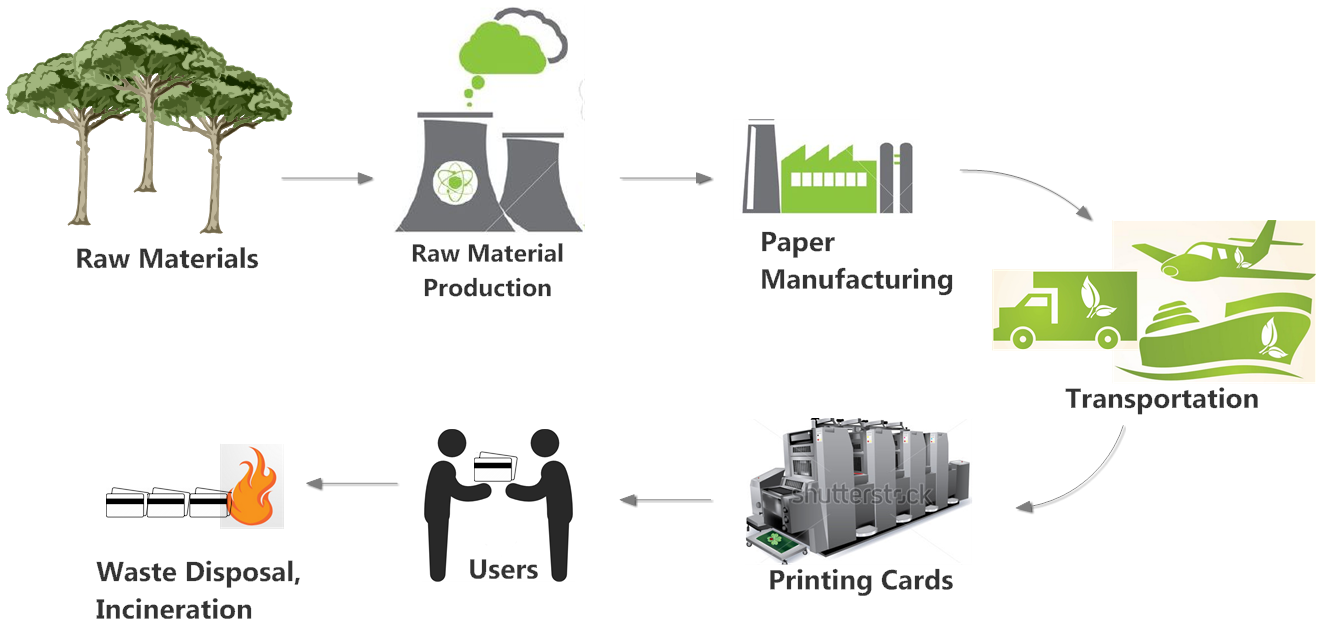
\includegraphics[width=\linewidth]{PBCSystem1.png}
\label{PBCSystem}
\caption{PBC system}\vspace*{-6pt}
\endminipage\hfill
\minipage{0.40\textwidth}
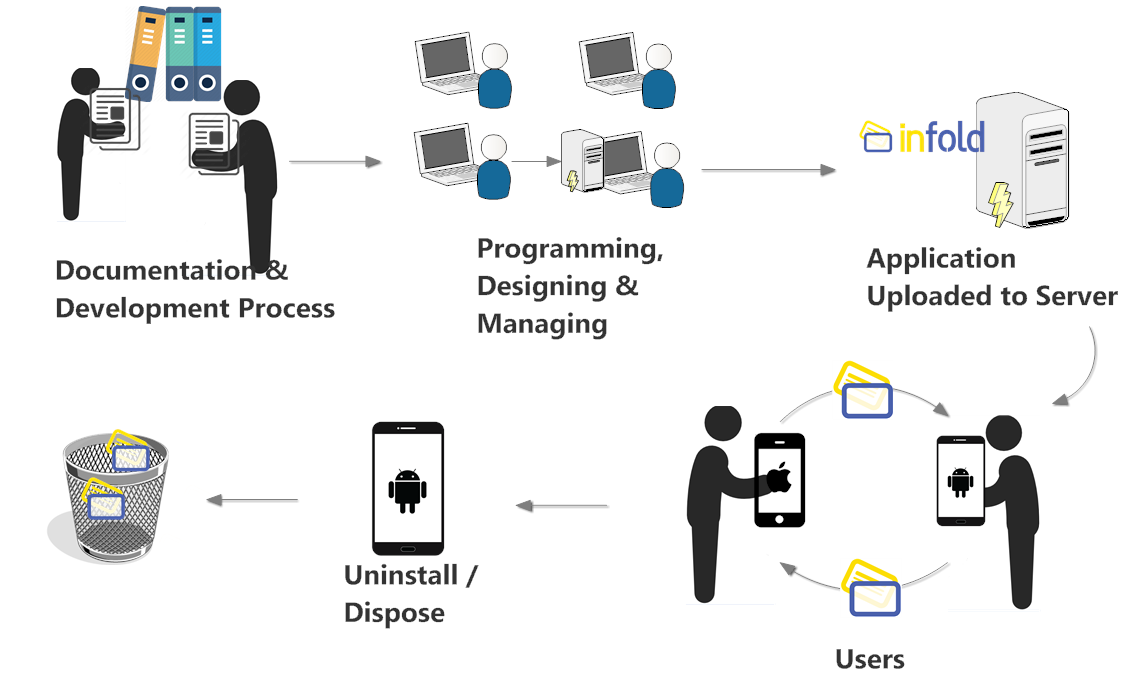
\includegraphics[width=\linewidth]{DBCSystem.png}
\label{DBCSystem}
\caption{DBC system}\vspace*{-6pt}
\endminipage\hfill
\end{figure}

The DBC software refers to a mobile application that facilitates the exchange of information packets between two or more customers through an Internet infrastructure including database servers and smartphones. Although there exist a variety of DBC software such as Card Flick, CamCard, Snapdat, One Card, Flextown, none of them fulfill the purpose and assumptions made in this study. In the scope of this research, the mobile application Infold was chosen as a DBC software, more specifically its version 0.1, which was developed specifically for the purposes of this study. Unlike the aforementioned alternatives, it supports only a single functionality, which is the creation and exchange of digital business cards and satisfies all the assumptions considered in this paper. A more detailed explanation of DBC and PBC systems is covered in subsections \ref{DBCBoundary} and \ref{PBCBoundary}.



\section{Method}

Life cycles of the two studied systems in this paper have been separately modeled in accordance with IS0 14040 LCA methodology. A two-stage cradle-to-grave life cycle analysis has been applied to PBC and DBC systems for identifying and evaluating life cycle impact categories as well as  total energy consumption, GHG emissions and toxic releases. The first stage (screening analysis) relies on the EIO approach that is capable of determining the principal sectors requiring more thorough analysis as well as providing a general evaluation of energy demand and environmental burdens associated with the studied systems. In LCA analysis it is of great importance to conserve the specificity of the studied systems or products. Due to limitations of the EIO approach, these concerns were not considered while performing the screening analysis. Therefore, two-stage analyses were conducted for gaining more comprehensive and reliable results. The second stage is based on the ISO LCA methodology and aims at providing a comprehensive examination and quantification of life cycle impact categories and burdens considering the findings from the first stage.

\subsection{General Assumptions}\label{Generalassume}
To compare DBC and PBC systems, some general assumptions were required which apply to both stages of this LCA analysis and are detailed below.

\begin{itemize}[]
\item The customer in this paper is identified as a person who possesses a PBC or uses the DBC software for creating and exchanging business cards.
\item Assuming that each company prints business cards annually, the lifetime considered for exhausting all business cards is one year.
\item PBC system scope is only a single functionality, that is the exchange of business cards, whereas DBC software could have multiple functionality such as exchange, management, broadcast, copy and translation of business cards. For simplicity and equivalent comparison between DBC and PBC systems, other functionality of these systems are not taken into consideration. This makes the complexity of allocation and multifunctionalilty of DBC system to be easily avoided.
\item The utilized energy during operation of the DBC software was measured using powerTutor mobile application (approximately 0.002778 Wh/exchange). The powerTutor was built by Google Inc. in collaboration with University of Michigan \cite{zhang2010accurate}. In fact, the measured energy usage is an upper bound.
 \item Since each DBC has an average size of 10 KB, then each one to one exchange between two customers is an exchange of 40 KB data over the Internet which includes the information packet header's size. From \cite{Moshnyaga:2013}, its assumed that 1 MB of traffic across the Internet takes 5.9 Wh which includes cooling, UPS, wiring, broadband routers, telephone lines. From \cite{EnergyDownload}, its assumed that the server and networking equipment consume 2.6 Wh/MB, cooling and losses contribute additional 1.3 Wh/MB, embedded infrastructure energy uses 0.9 Wh/MB and the DSL Access Multiplexers (DSLAMs) and phone line require 1.1 Wh/MB. Therefore, the overall required energy consumption for each one to one exchange is up to 5.9 Wh/MB,  which is an upper bound.
\item The energy consumption from the DBC software update has not been considered because the functionality of the product is already fulfilled and there is no need for the customer to update his/her software.
\item The dedicated effort and cost for the development of the future updates of the DBC software is not taken into account.
\item The environmental impact from the production of server used in DBC system is considered since it is allocated specifically for the purposes of DBC software.
\item Servers usually have more than one year lifetime, however, the considered production cost of server used in the DBC system is for one year.
 \item An upper-bound energy consumption of server used in the DBC system was estimated to be 45 Wh based on the data from the hosting provider (Digital Ocean).
\item For simplicity and fair impact assessment the environmental impact originated from the production and manufacturing of a smartphone used in DBC system has not been taken into account, since it is not utilized specifically for the DBC software and should be amortized over the active smartphone applications which significantly varies among customers.
\item Due to a highly complex structure and diverse functionality of the Internet, this paper ignores all the environmental impacts and energy depletion associated with the components and devices in the Internet except the ones that are allocated specifically for exchanging DBC over the Internet.
\end{itemize}

\subsection{Functional Unit}\label{sec:FunctionalUnit}

A functional unit defines the foundation of LCA for comparing two or more products. All the data collected in the inventory will be dependent on the defined functional unit. In this study, DBC and PBC products are compared on a one to one basis. An exchange of each of them between two customers requires an exchange of two business cards or two equivalent information packets. It is worth mentioning that in DBC system, a customer can broadcast a single information packet representing the business card to other customers which is much more efficient in terms of bandwidth consumption rather than a one to one exchange. Even though the latter functionality is energy beneficial to DBC system, but for the unbiased comparison, it is not considered since there is no feasible way to broadcast in PBC system.\\

In order to obtain a comprehensive and accurate picture of DBC and PBC system's life cycle impacts, two cases of functional units were considered; a case of 1000 exchanges between customers in PBC and DBC systems, that is production and exchange of 2000 PBC and DBC respectively and a case of 33000 exchanges between customers in PBC and DBC systems or production and exchange of 66000 PBC and DBC respectively. The latter case is a real world scenario based on the data and statistics regarding annually utilized business cards provided by the Human Resource department at Masdar Institute of Science and Technology. 

\subsection{PBC System Boundary} \label{PBCBoundary}
Life cycle model of the PBC system is composed of five major stages which, along with their model elements, are listed in Table \ref{PBCboundary}. A brief description of each stage and corresponding model elements is provided below.

A PBC is generally composed of paper and ink. These components are acquired from chemical manufacturing and paper manufacturing processes which require natural resources. Paper manufacturing sector is not available in some countries, hence the transportation of paper based products could be included in the according stage. After obtaining the paper with a suitable quality, thickness and predetermined size, PBC design procedure begins followed by the printing stage. Hereafter, already made PBC are collected and stored in the appropriate facilities and then delivered to the customers. Then costumers exchange PBC during various events including conferences and meetings. When the useful life of the PBC is expired, the product is disposed as a municipality waste or incinerated.

\subsection{DBC System Boundary}\label{DBCBoundary}

DBC system boundary is quite different from the system boundaries of traditional industrial products. The life cycle model of the DBC system considered in this paper is similar to the one in \cite{Moshnyaga:2013, moshnyaga2013assessment} and along with the model elements is detailed in Table \ref{DBCboundary}. A brief description of each stage and corresponding model elements is provided in consequent paragraph.\\

The DBC system has no raw materials as an input to the system. The manufacturing stage of the DBC system involves typical software engineering process, as well as tools and facilities used by the corresponding personnel in charge of the development of the DBC software. The aforementioned facilities and tools include but are not limited to custom software like Eclipse IDE, Android Studio and equipment like PCs, Air Conditioners, UPSs, printers, and lighting. After the manufacturing stage, the DBC software is deployed online so that it is accessible for customers. Once the DBC software is downloaded and installed on a smartphone, a customer starts using the software for creating and exchanging DBC, during which the according information packets are routed through the Internet. Further environmental burdens are associated with the production and disposition of the server. Finally, end-of-life stage is simply uninstalling the DBC software from a smartphone. 

\begin{table}[h]
\caption{Life Cycle Model of the DBC System}
\begin{tabular*}{\hsize}{@{\extracolsep{\fill}}lllll@{}}
\toprule
\textbf{Life Cycle Stage} & Manufacturing & Distribution & Use & End-of-Life\\
\colrule
\textbf{Model Elements} &   Software Engineering &  DBC Software Installation  & Server Production & DBC Software Uninstallation\\

 & DBC Software Development &   & Server Disposal  & \\
  &  Facility Infrastructure  &   & Smartphone Use &   \\
    &  &   & File Transfer &   \\
    &  &   & DBC Exchange &   \\
\botrule
\end{tabular*}
\label{DBCboundary}
\end{table}
\vspace{-0.6cm}
\begin{table}[h]
\caption{Life Cycle Model of the PBC System}
\begin{tabular*}{\hsize}{@{\extracolsep{\fill}}llllll@{}}
\toprule
\textbf{Life Cycle Stage} & Material Production & Manufacturing  & Distribution & Use & End-of-Life\\
\colrule
\textbf{Model Elements} &   Paper Production &  PBC Creation and Printing & Facility Infrastructure & PBC Exchange & PBC Disposal \\
 &  Ink Production &   & Collection and Storage &  &  \\
  &   &   & PBC Delivery &  &  \\
\botrule
\end{tabular*}
\label{PBCboundary}
\end{table}
\vspace{-0.4cm}
\section{Screening Analysis} \label{ScreeningLCA}

As a first stage of this LCA study a screening of the environmental impacts and energy consumption has been carried out by applying EIO LCA methodology to PBC and DBC systems. The analysis was performed using Carnegie Mellon EIO LCA online tool, which uses U.S. data from 2002 \cite{Mellon}. The monetary expenses were calculated for DBC and PBC systems in both cases of functional units and served as an input to EIO LCA. The calculations for the DBC system shown in Table \ref{PBCcalc} are based on the assumption that electricity price is 0.5 USD per KWh. For the PBC system's calculations it was assumed that the average cost of printing 200 standard business cards is 50 USD. This assumption was based on the extensive observations on the price statistics offered by various U.S. based business card printing services.

\begin{table}[h]
\label{PBCcalc}
\caption{Monetary Expenses of the DBC system}
\begin{tabular*}{\hsize}{@{\extracolsep{\fill}}ll@{}}
\colrule
\textbf{Production of a server} & 240 USD annually \\
\textbf{Production of a software}  &   8000 USD \\
(all inclusive cost considering expenses associated with the corresponding personnel and facilities) &  \\
\textbf{Server energy consumption} &  45 Wh hence, 394.2 KWh annually \\
\textbf{Energy consumption from software installation} (for 1000 exchanges) &  236 Wh \\
\textbf{Smartphone energy consumption} (for 1000 exchanges) &  2.778 Wh \\
\textbf{Total energy and monetary expenses} (software installation + smartphone + server) &  394.439 KWh hence, total \\
(for 1000 exchanges) & expenses are 197.22 USD \\
\textbf{Total energy and monetary expenses} (for the case of 33000 exchanges) & 406.1389 KWh,  hence total  \\
& expenses are 203.06945 USD  \\
\botrule
\end{tabular*}
\end{table}
\vspace{-0.5cm}
\subsection{Results}
Results of a first screening of the environmental impacts and energy consumption of PBC and DBC systems for both cases of functional units i.e. 1000 and 33000 exchanges are presented in Figure \ref{screen1}, Figure \ref{screecn3Sectors} and Figure \ref{screecn4Sectors}. The toxic releases shown in Figure \ref{screen1} refer to different environments such as surface and under water, land, air and include metals and non metals. Economic sectors that have less than 1\% contribution to the aggregate GHG emissions are represented in a single compound sector entitled "Other sectors" in Figure \ref{screecn3Sectors} and Figure \ref{screecn4Sectors}. For the case of 1000 exchanges Figure \ref{screen1} shows that the PBC system has less environmental impact and energy consumption compared to the DBC system. On the contrary, the leftmost graph in Figure \ref{screen1} clearly shows that for the case of 33000 exchanges the DBC system is far more environmentally friendly than the PBC system emitting almost 3 times less amount of GHGs than the PBC system. Likewise, the PBC system's consumed energy and toxic releases are nearly 4 and 10 times higher than those of the DBC system respectively. The results shown in Figure \ref{screecn3Sectors} indicate that GHG emissions of the PBC system are mainly driven by two sectors, namely power generation and supply (38\%) and paper mills (15\%), followed by truck transportation (5\%), oil and gas extraction (5\%) and printing (5\%) sectors having relatively small impacts. This implies that the large portion of the GHG emissions of the PBC system are due to the electricity usage and paper production during the manufacturing and material production life cycle stages. Unlike the PBC system, where GHG emissions are more or less evenly distributed among the sectors the dominating GHG emitting sector in the DBC system is power generation and supply, which demands 85\% of the cumulative GHG emissions as shown in Figure \ref{screecn4Sectors}. Hence, it could be concluded that GHG emissions originated from the electricity consumption and server equipment production during the manufacturing and use stages of the DBC system life cycle significantly alter its GHG emissions. 

\begin{figure}[t]
\minipage{0.52\textwidth}
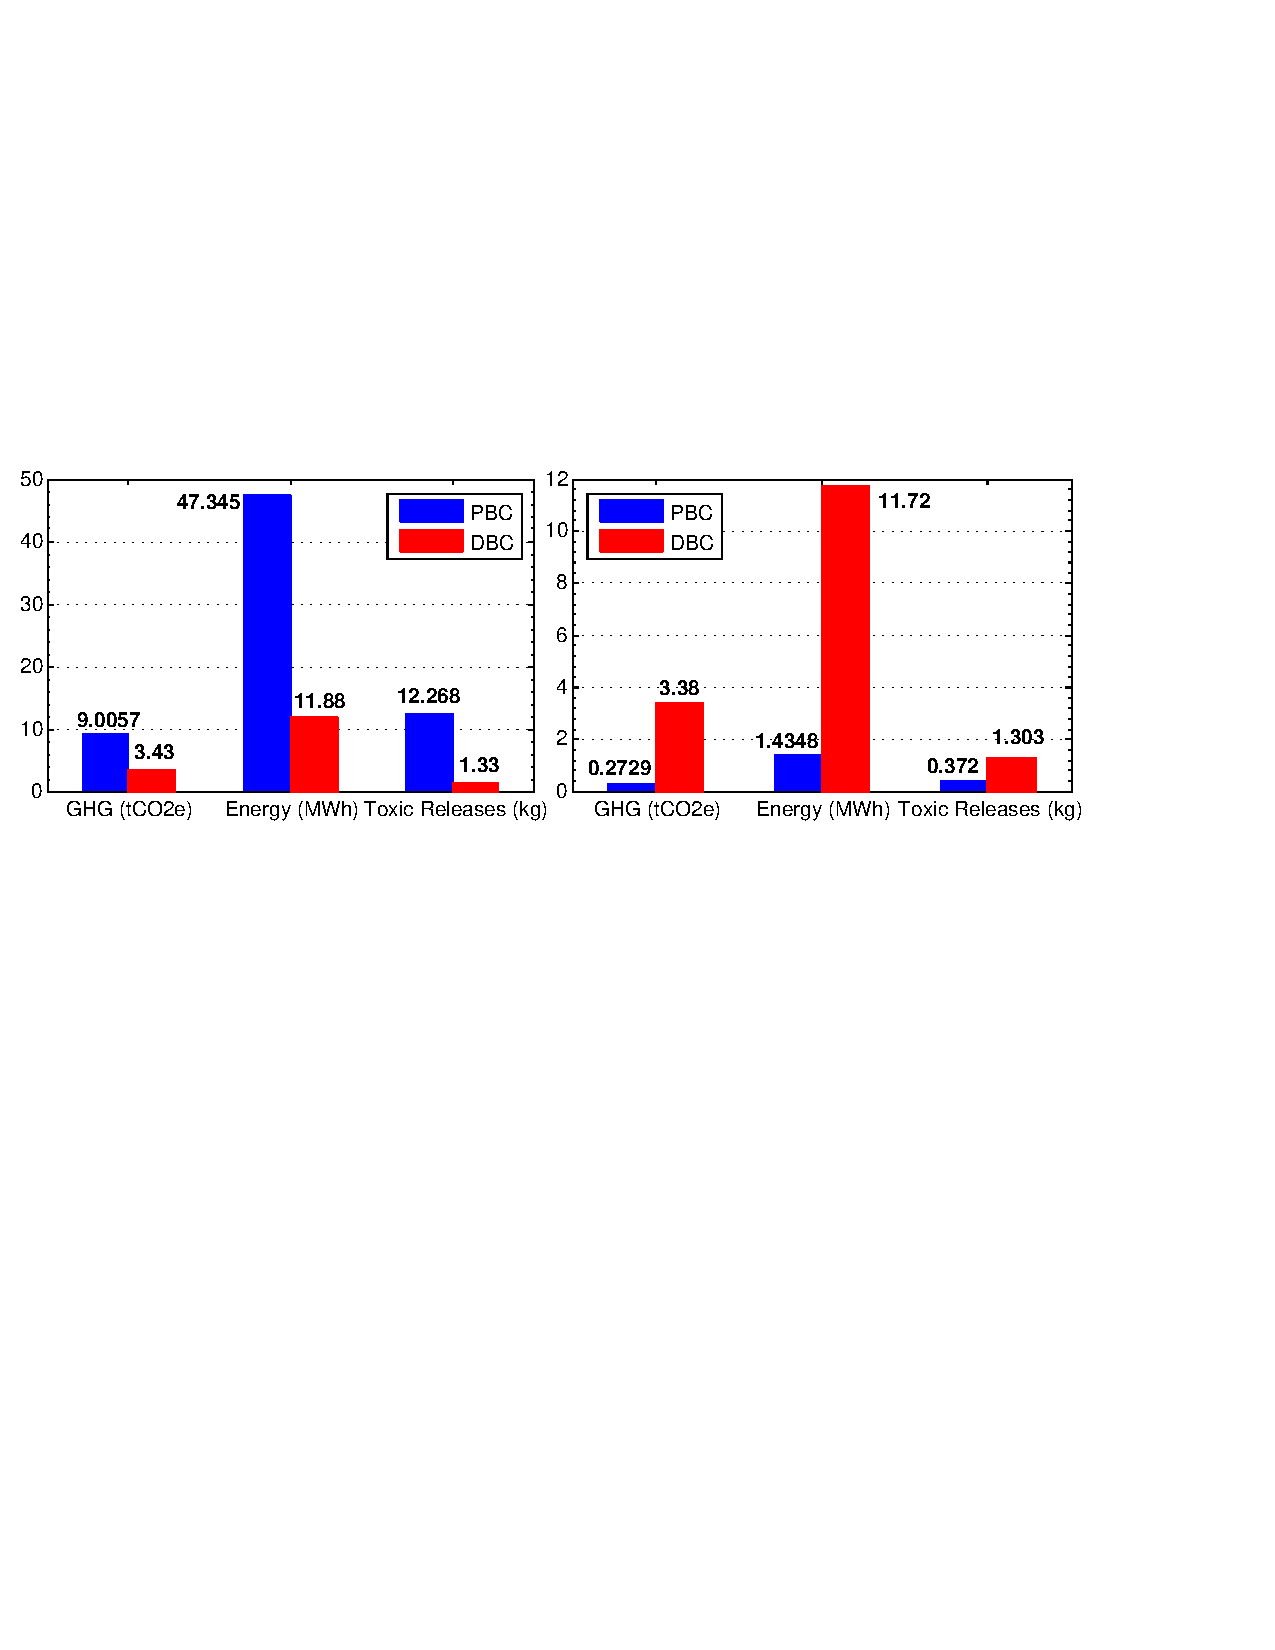
\includegraphics[width=\linewidth]{sf.pdf}
\caption{Environmental impacts and energy consumption of PBC and DBC systems for 1000 and 33000 exchanges of on right and left respectively}
\label{screen1}
\endminipage\hfill
\minipage{0.42\textwidth}
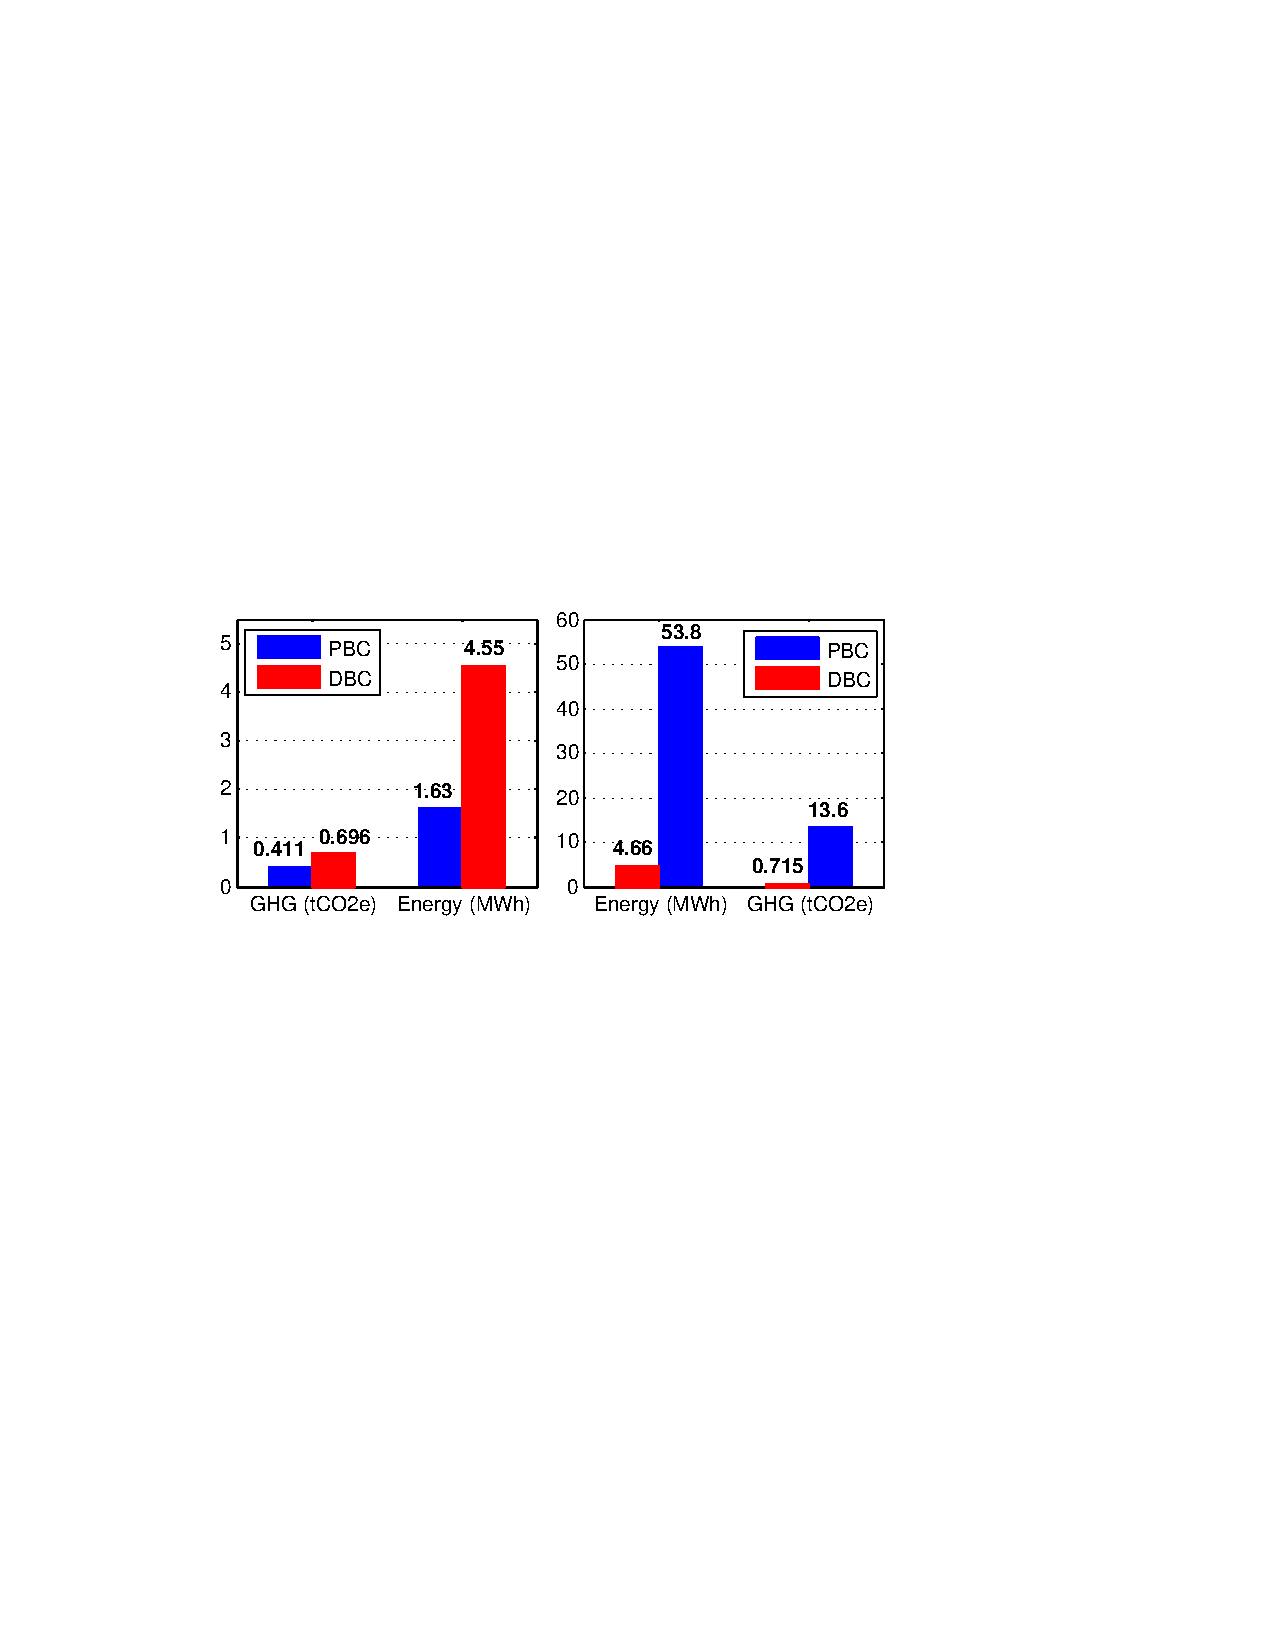
\includegraphics[width=\linewidth]{fs.pdf}
\caption{GHG emissions and energy consumption of PBC and DBC systems for 1000 and 33000 exchanges of on left and right respectively}
\label{fig:onescore}
\endminipage\hfill
\end{figure}


\begin{figure}[t]
\minipage{0.51\textwidth}
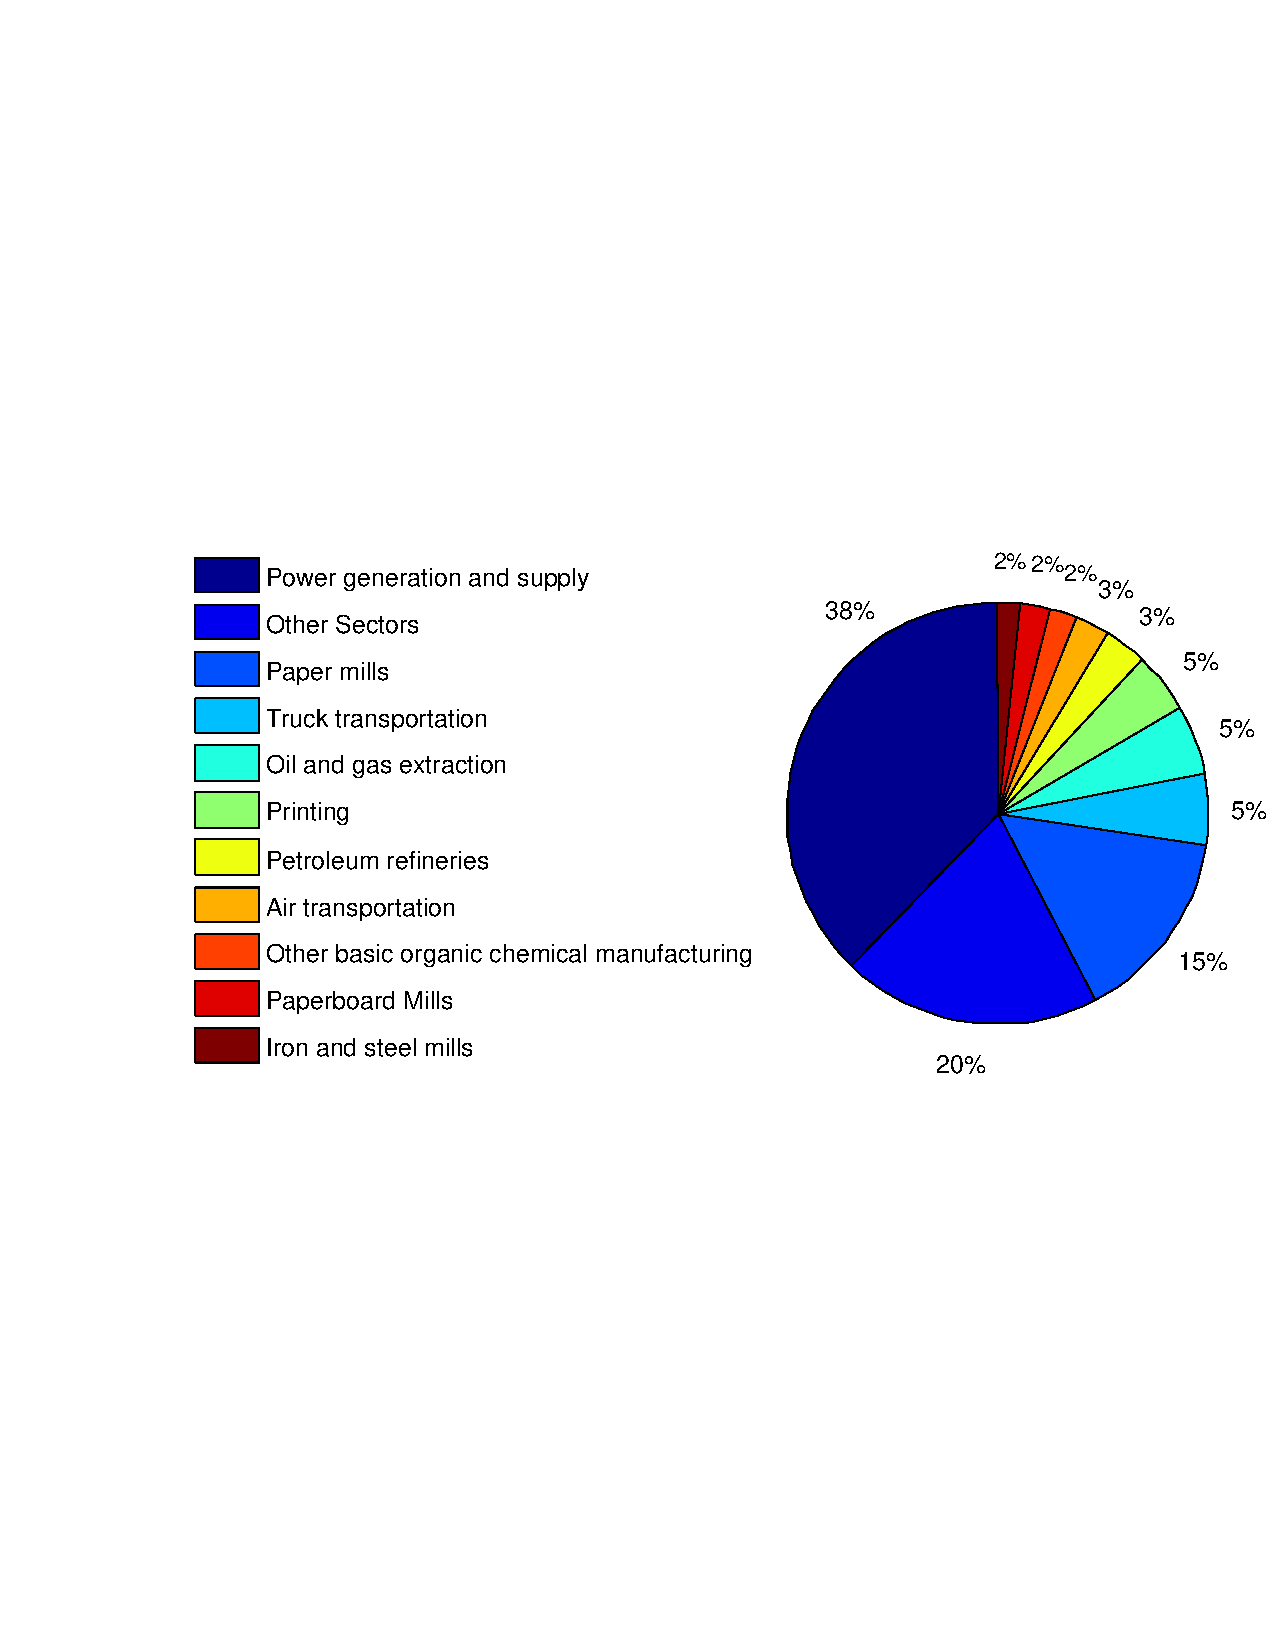
\includegraphics[width=\linewidth]{f.pdf}
\caption{GHG emissions of the PBC system by economic sectors}
\label{screecn3Sectors}
\endminipage\hfill
\minipage{0.44\textwidth}
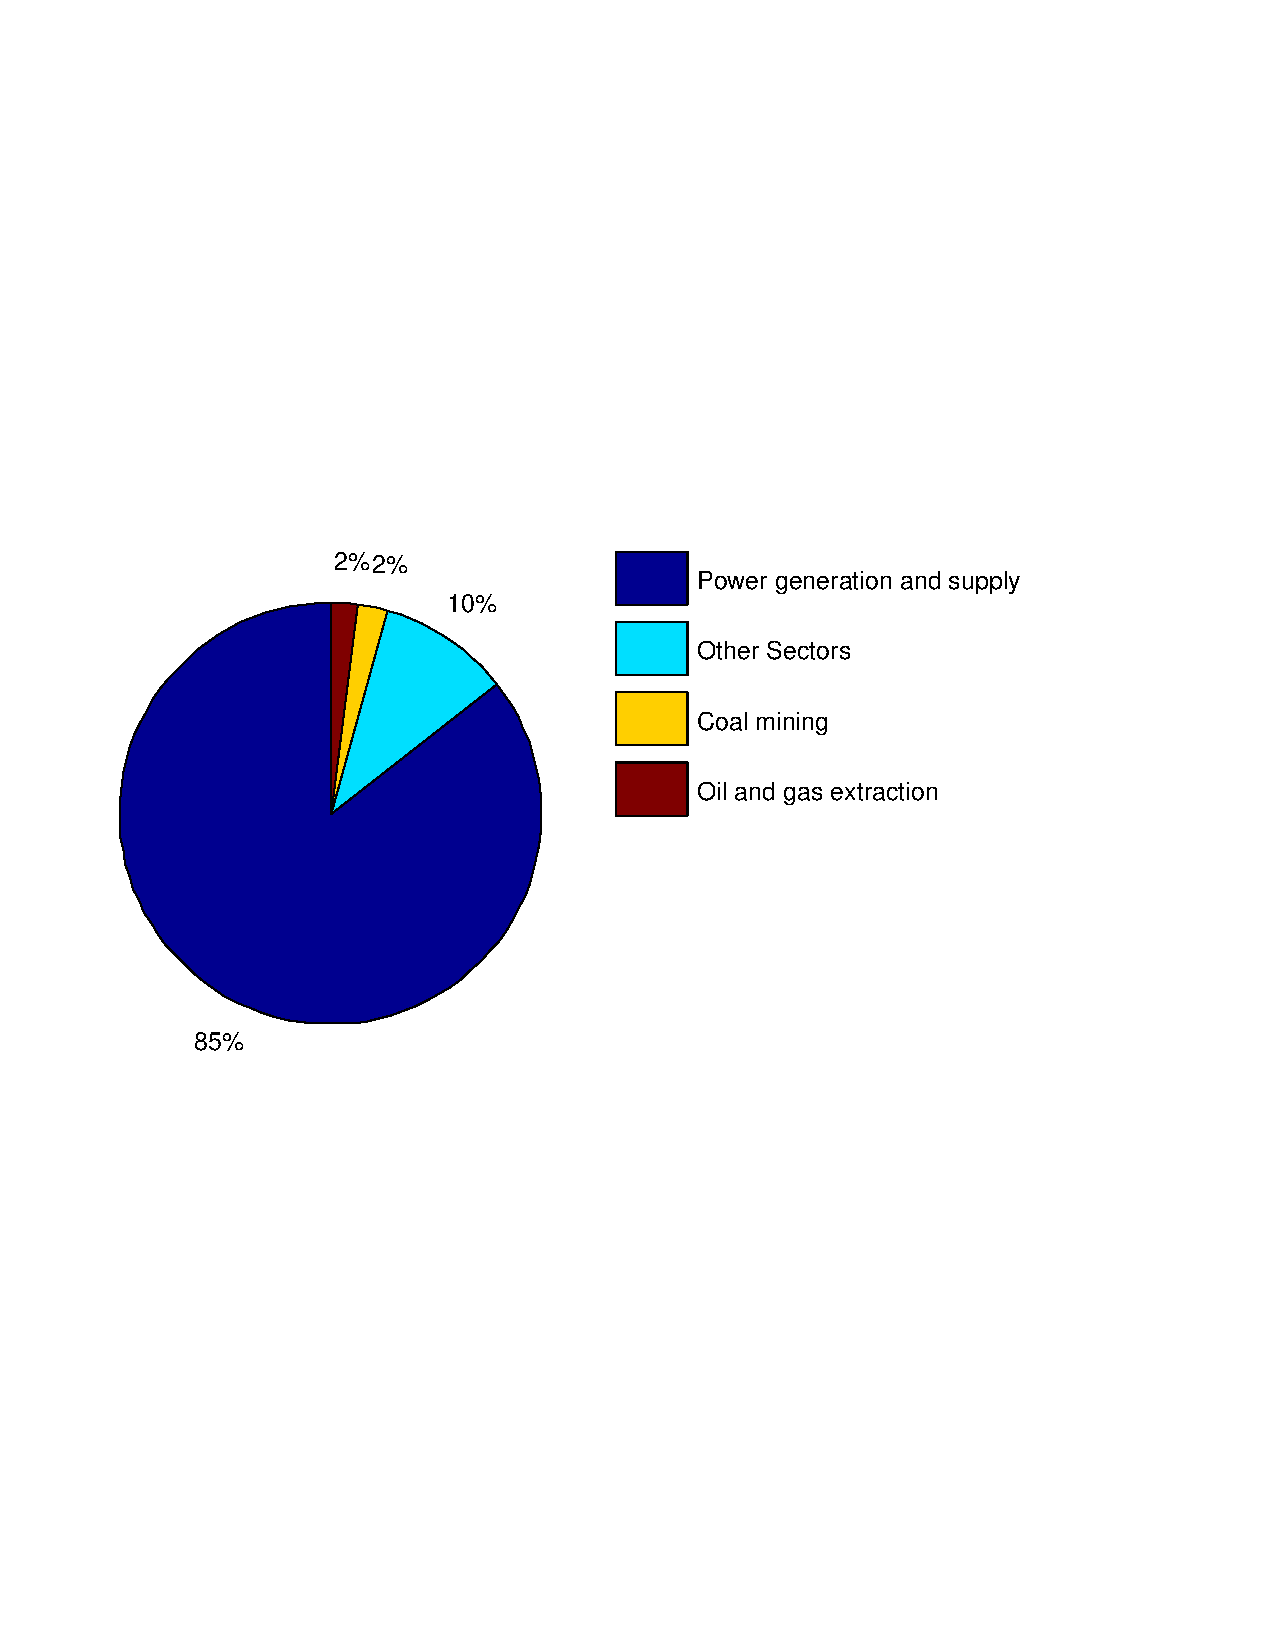
\includegraphics[width=\linewidth]{g.pdf}
\caption{GHG emissions of the DBC system by economic sectors}
\label{screecn4Sectors}
\endminipage\hfill
\end{figure}


\section{Second Stage Analysis}
An in-depth analysis and quantification of environmental impact categories and life cycle burdens has been conducted for the second stage of this LCA analysis using SimaPro 7.3 software with Ecoinvent 3.1 database based on U.S. data from 2004.

\subsection{Life Cycle Inventory}
Data collection and calculations performed in the Life Cycle Inventory (LCI) phase of this study, which quantify associated inputs and outputs in the PBC and DBC systems are detailed below as well as provided previously in subsection \ref{Generalassume}. 

Dimensions of the standard PBC were considered to be 3.37 inches in width and 2.125 inches in height based on ISO/IEC 7810 Identification cards' standard.  The standard quality business card paper weight was considered to be 350 g per $m^2$. Considering the latter two facts, the weight of one PBC was estimated to 1.63824 g. When printing a PBC some space of paper is left empty to avoid overlapping between cards. This is usually referred as bleed space which is 0.125 of the height and width of PBC. Hence the weight of a single PBC has been considered to be 1.8194 g. The server used in the DBC system for facilitating exchanges has the following specifications; Intel(R) Xeon(R) CPU E5-2630L v2 @ 2.40GHz, 1GB Ram, 30GB SSD Hard Disk.\\

LCI results for the PBC and DBC systems for both cases of functional units are shown in Figure \ref{fig:onescore}. For brevity life cycle impacts other than GHG emissions and energy consumption are not discussed. The results are in confirmation with the previous findings of screening analysis. However, as could be expected, there are significant numerical differences between them. More specifically, for the case of 1000 exchanges, the screening analysis reveals a considerable difference between environmental impacts and energy consumption of DBC and PBC systems in favor of the latter. Nonetheless, LCI results show that for the case of the functional unit being 1000 exchanges the DBC system emitted only about 1.7 times the amount of CO2 equivalent emissions than the PBC system. Likewise, the Energy consumption of the DBC system being 4.55 MWh is only three times higher than the energy demand of the PBC system. Moreover, for the case of 33000 exchanges, the difference between LCI and EIO LCA results are more noticeable as could be seen from Figure \ref{fig:onescore}. The difference between results may imply the following: (1) life cycle burdens of the DBC system largely depend on the fixed impact which is nothing else but the burdens caused by development of the DBC software and manufacturing of server hardware (2) life cycle impacts of the PBC system heavily depend on the number of exchanges (3) rate of growth of the life cycle impacts of the PBC system based on the number of exchanges is remarkably higher than that of the DBC system.

\begin{table}[h]
\caption{Environmental impacts of PBC and DBC systems for 1000 and 33000 exchanges in terms of Ecopoints}
\begin{tabular*}{\hsize}{@{\extracolsep{\fill}}llllll@{}}
\toprule
\multicolumn{2}{l}{\multirow{2}{*}{\textbf{}}} & \multicolumn{2}{l}{\textbf{1000 Exchnages}} & \multicolumn{2}{l}{\textbf{33000 Exchanges}} \\ 
\colrule
\multicolumn{2}{l}{} & \textbf{DBC} & \textbf{PBC} & \textbf{DBC} & \textbf{PBC} \\
\multicolumn{2}{l}{\it{Total}} & \it{0.317} & \it{0.279} & \it{0.326} & \it{9.21} \\ 
\multicolumn{2}{l}{Carcinogens} & 0.00106 & 0.00816 & 0.00108 & 0.0269 \\ 
\multicolumn{2}{l}{Non-carcinogens} & 0.00886 & 0.0751 & 0.00909 & 2.48 \\ 
\multicolumn{2}{l}{Respiratory inorganics} & 0.108 & 0.0713 & 0.111 & 2.35 \\
\multicolumn{2}{l}{Ionizing radiation} & 0.00308 & 0 & 0.00317 & 0 \\
\multicolumn{2}{l}{Ozone layer depletion} & 4.60E-05 & 2.11E-04 & 4.80E-05 & 0.00697 \\ 
\multicolumn{2}{l}{Respiratory organics} & 5.27E-05 & 0.000294 & 5.80E-05 & 9.72E-03 \\
\multicolumn{2}{l}{Aquatic ecotoxicity} & 0.00748 & 0.000651 & 0.00769 & 2.15E-02 \\
\multicolumn{2}{l}{Terrestrial ecotoxicity} & 0.00684 & 0.0401 & 0.00701 & 1.32 \\ 
\multicolumn{2}{l}{Terrestrial acidification} & 0.00127 & 0.00089 & 0.00131 & 0.0294 \\ 
\multicolumn{2}{l}{Land occupation} & 0.00204 & 0.00229 & 0.0021 & 0.0756 \\ 
\multicolumn{2}{l}{Global warming} & 0.0703 & 0.0415 & 0.07222 & 1.37 \\ 
\multicolumn{2}{l}{Non-renewable energy} & 0.108 & 0.0387 & 0.111 & 1.28 \\ 
\multicolumn{2}{l}{Mineral extraction} & 2.89E-04 & 0.000001918 & 2.96E-04 & 6.33E-05 \\ 

\botrule
\end{tabular*}
\label{PBCandDBCexchanges}
\end{table}
\vspace{-0.5cm}
\subsection{Life Cycle Impact Assessment}
Life Cycle Impact Assessment (LCIA) phase of this LCA study focuses on revealing and assessing environmental impacts and impact categories of PBC and DBC systems throughout their life cycle. LCIA results presented in Table \ref{PBCandDBCexchanges} represent a single score comparison between both systems based on the conversion of LCI results to Ecopoints. Ecopoints are a composite measure of the overall environmental impact of any material, product or service.\\

As could be noticed from Table \ref{PBCandDBCexchanges} different cases of functional units lead to different results. The relations between DBC and PBC systems in terms of environmental impact alters when changing the functional unit. For the case of the functional unit being 1000 exchanges environmental impact of the PBC system is slightly lower than that of the DBC system. Specifically, the DBC system emitted nearly two times higher quantities of global warming emissions and chemicals  related to acidification than the PBC system. In addition the DBC system emitted nearly twenty times higher ozone depleting substances that the PBC system. Whereas, when it comes to raw materials the PBC system required almost 10 times higher amount of raw materials than the DBC system. These can be explained by the initial high impacts posed by the manufacturing and use stages of the DBC system life cycle.\\

In contrast, environmental burdens caused by the DBC system are significantly lower compared to those of the PBC system for the case of the functional unit being 33000 exchanges. More precisely, the overall environmental impact of the PBC system is about 30 times higher than that of the DBC system. Furthermore, the PBC system has far worse impacts in almost all environmental categories than the DBC system. This is because the manufacturing and use stages of the DBC system life cycle have been amortized over high number of exchanges. Considering the findings from both stages of this LCA analysis, it is safe to assume that up to certain limit the higher the number of exchanges, the more amortized are the impacts caused by the manufacturing and use stages of the DBC system life cycle.

\section{Conclusions}

In this paper the findings of a comparative life cycle assessment of paper-based and software-based business card systems are presented. For reliable and accurate results, two-stage cradle-to-grave analysis of environmental impacts and impact categories of the two systems is conducted for two cases of functional units. In addition, energy consumption, GHG emissions and toxic releases of the two systems have been analyzed and quantified. Under the considered assumptions, for the case of a small scale functional unit the paper-based business card system is more environmentally friendly and economical in terms of energy consumption. Nevertheless, for the case of a large scale (real world scenario) functional unit the software-based business card system has significantly less environmental impact and energy utilization compared to the paper-based system. The results indicate that life cycle burdens of the software-based business card system are mainly driven from
the electricity consumption and server equipment production
during the manufacturing and use stages of its life cycle. Similarly, electricity usage and paper production during the manufacturing and material production life cycle stages of the paper-based business card system are the major contributors to its life cycle impacts. Sensitivity analysis of the results is a subject to future work. This study is not meant to label or discourage paper-based or software-based business cards. Instead, the findings of this study provide industry and consumers with adequate information for considering environmentally aware decisions
regarding the two systems. Furthermore, this paper contains information regarding software life cycle assessment that could be useful for the development of sustainable technologies and green software. 

\section*{Acknowledgment}

This study was conducted under the support and funding of Masdar Institute of Science and Technology.

\bibliography{reference}
\bibliographystyle{model3a-num-names}

\end{document}

%%
%% End of file `procs-template.tex'.
